\section{Raw covariance and projection in Experiment 8}\label{app:projection}
The raw covariance map and the matrix used in NLL are distinct. This illustrative seed-0 diagnostic uses the same prescribed grid as the main coefficient figures. Projection is the existing symmetrization/eigenvalue floor at $10^{-3}$, whereas the smallest true instantaneous eigenvalue is $10^{-8}$. No floor was tuned for the plot.
\begin{figure}[htbp]\centering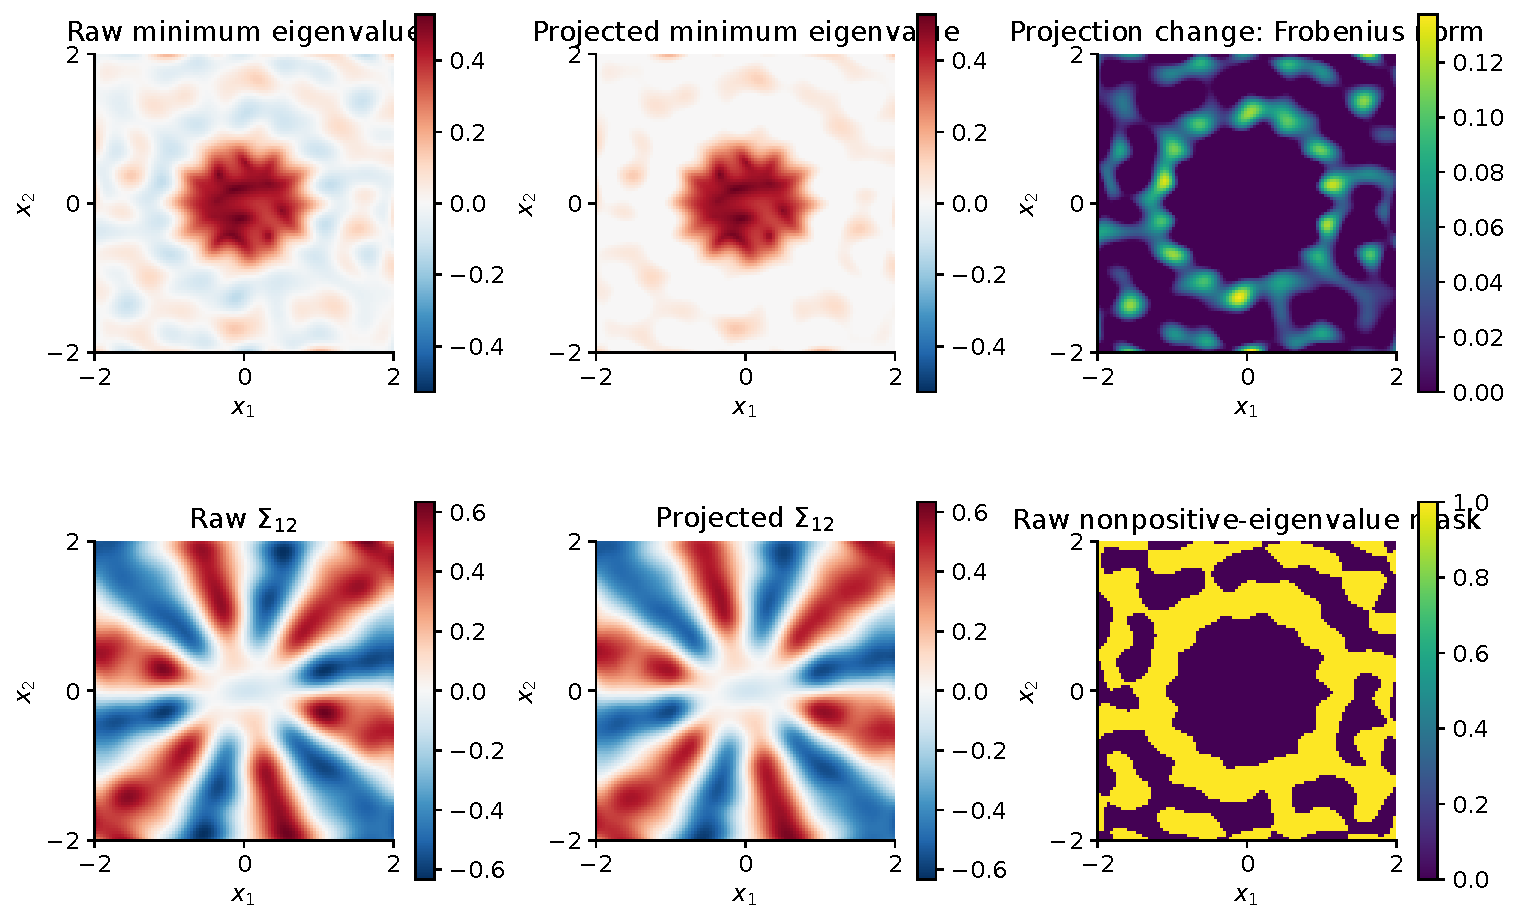
\includegraphics[width=\linewidth]{../figures/ex8_seed0_projection.pdf}
\caption{Seed-0 ARFF: raw and projected smallest eigenvalues, projection-change norm, raw/projected off-diagonal entry, and raw nonpositive-eigenvalue mask. Raw/projected eigenvalue and entry pairs have shared scales. Projection does not repair the raw coefficient estimate retroactively. Grid rates are not the production test-set rates.}\end{figure}

\section{Complete sample-size sensitivity and numerical records}\label{app:sensitivity}
\begin{figure}[htbp]\centering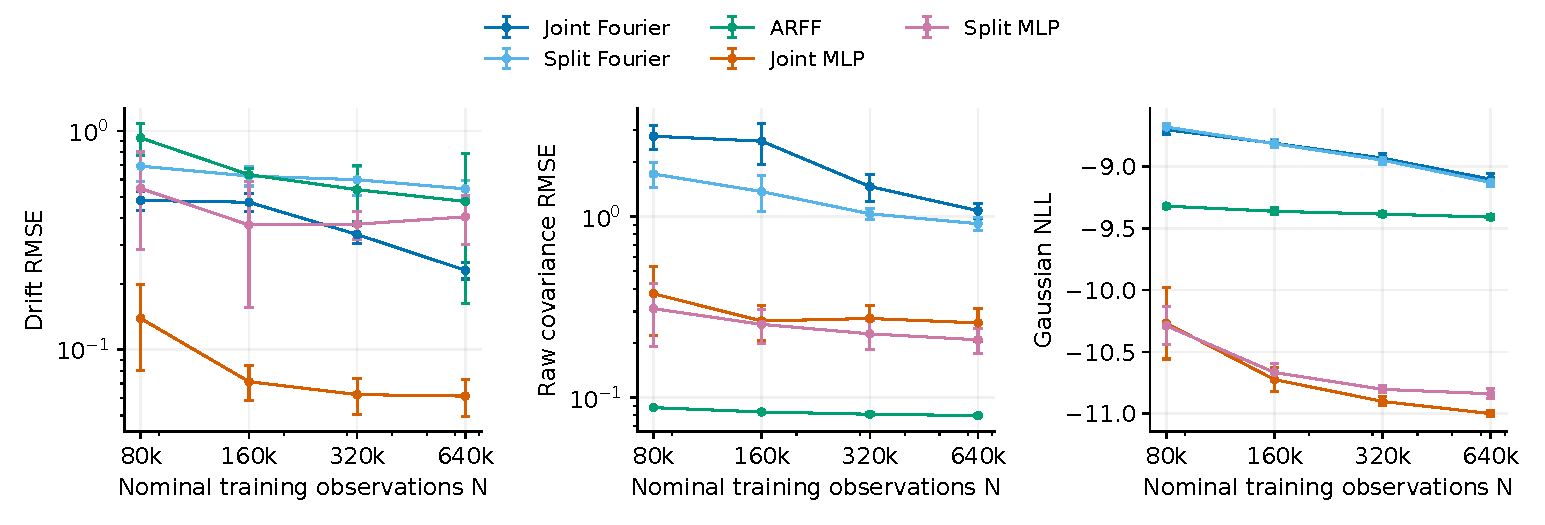
\includegraphics[width=\linewidth]{../figures/N.pdf}\caption{Completed Ex8 sample-size study at $K=1024,h=10^{-4}$: ten fitting seeds on nested training data, with shared validation/test states. Means and sample SDs describe fitting variation, not independent dataset variation.}\end{figure}
The four N points, nine lag points and five capacity points comprise 200,450,250 method/point/seed records, respectively. Their shared 50-record anchor means 800 distinct records, not 900 independent experiments. The 30-seed baseline is separate. Both validation equivalence screens failed; capacity uses the predetermined fallback rather than an established approximation-dominated regime. Full N/h/K and raw-SPD tables follow.
\small
\begin{longtable}{llrrr}\caption{N study: test mean $\pm$ sample SD over ten fitting seeds. Raw covariance errors; all points retained.}\\\toprule Method & Point & Drift RMSE & Raw covariance RMSE & NLL\\\midrule\endfirsthead\toprule Method & Point & Drift RMSE & Raw covariance RMSE & NLL\\\midrule\endhead
Joint Fourier & 80000 & $0.4817\pm 0.0501$ & $2.782\pm 0.4231$ & $-8.704\pm 0.03926$\\
Joint Fourier & 160000 & $0.4723\pm 0.04396$ & $2.613\pm 0.6617$ & $-8.813\pm 0.03376$\\
Joint Fourier & 320000 & $0.3363\pm 0.03173$ & $1.468\pm 0.2504$ & $-8.934\pm 0.03365$\\
Joint Fourier & 640000 & $0.2308\pm 0.02035$ & $1.079\pm 0.1059$ & $-9.105\pm 0.04537$\\
Split Fourier & 80000 & $0.6909\pm 0.1052$ & $1.721\pm 0.2708$ & $-8.682\pm 0.02906$\\
Split Fourier & 160000 & $0.6226\pm 0.06222$ & $1.376\pm 0.3082$ & $-8.817\pm 0.03064$\\
Split Fourier & 320000 & $0.599\pm 0.09298$ & $1.038\pm 0.07346$ & $-8.95\pm 0.0355$\\
Split Fourier & 640000 & $0.5436\pm 0.04761$ & $0.9144\pm 0.07123$ & $-9.13\pm 0.03469$\\
ARFF & 80000 & $0.9297\pm 0.1535$ & $0.08826\pm 0.00116$ & $-9.322\pm 0.01596$\\
ARFF & 160000 & $0.6316\pm 0.04304$ & $0.08352\pm 0.00103$ & $-9.363\pm 0.02774$\\
ARFF & 320000 & $0.5391\pm 0.1531$ & $0.08115\pm 0.0013$ & $-9.386\pm 0.01878$\\
ARFF & 640000 & $0.4763\pm 0.3129$ & $0.07976\pm 0.001234$ & $-9.411\pm 0.01881$\\
Joint MLP & 80000 & $0.1389\pm 0.05881$ & $0.3756\pm 0.1536$ & $-10.27\pm 0.289$\\
Joint MLP & 160000 & $0.07144\pm 0.01292$ & $0.2656\pm 0.0575$ & $-10.72\pm 0.09529$\\
Joint MLP & 320000 & $0.06234\pm 0.01154$ & $0.2742\pm 0.04925$ & $-10.9\pm 0.03649$\\
Joint MLP & 640000 & $0.06135\pm 0.01203$ & $0.2591\pm 0.05327$ & $-11\pm 0.02579$\\
Split MLP & 80000 & $0.5461\pm 0.2588$ & $0.3106\pm 0.118$ & $-10.29\pm 0.1525$\\
Split MLP & 160000 & $0.3719\pm 0.2158$ & $0.2543\pm 0.05389$ & $-10.67\pm 0.06984$\\
Split MLP & 320000 & $0.3749\pm 0.05553$ & $0.2256\pm 0.04057$ & $-10.8\pm 0.02846$\\
Split MLP & 640000 & $0.4052\pm 0.1033$ & $0.209\pm 0.03326$ & $-10.84\pm 0.04174$\\
\bottomrule\end{longtable}
\begin{longtable}{llrrr}\caption{h study: test mean $\pm$ sample SD over ten fitting seeds. Raw covariance errors; all points retained.}\\\toprule Method & Point & Drift RMSE & Raw covariance RMSE & NLL\\\midrule\endfirsthead\toprule Method & Point & Drift RMSE & Raw covariance RMSE & NLL\\\midrule\endhead
Joint Fourier & $2.5\times10^{-5}$ & $0.3259\pm 0.0349$ & $1.507\pm 0.2459$ & $-10.53\pm 0.04815$\\
Joint Fourier & $5\times10^{-5}$ & $0.2687\pm 0.03135$ & $1.273\pm 0.1626$ & $-9.83\pm 0.04447$\\
Joint Fourier & 0.0001 & $0.2308\pm 0.02035$ & $1.079\pm 0.1059$ & $-9.105\pm 0.04537$\\
Joint Fourier & 0.0002 & $0.2049\pm 0.03395$ & $0.9433\pm 0.08391$ & $-8.36\pm 0.04026$\\
Joint Fourier & 0.0004 & $0.139\pm 0.01799$ & $0.8228\pm 0.07923$ & $-7.593\pm 0.041$\\
Joint Fourier & 0.0008 & $0.1389\pm 0.01118$ & $0.7333\pm 0.06999$ & $-6.822\pm 0.03166$\\
Joint Fourier & 0.001 & $0.1393\pm 0.01692$ & $0.6938\pm 0.06811$ & $-6.558\pm 0.02712$\\
Joint Fourier & 0.0015 & $0.1166\pm 0.008672$ & $0.645\pm 0.07429$ & $-6.119\pm 0.02544$\\
Joint Fourier & 0.002 & $0.1032\pm 0.01297$ & $0.6147\pm 0.06438$ & $-5.78\pm 0.01732$\\
Split Fourier & $2.5\times10^{-5}$ & $1.395\pm 0.1083$ & $1.07\pm 0.1096$ & $-10.55\pm 0.03477$\\
Split Fourier & $5\times10^{-5}$ & $0.8385\pm 0.08578$ & $0.9949\pm 0.1184$ & $-9.841\pm 0.04611$\\
Split Fourier & 0.0001 & $0.5436\pm 0.04761$ & $0.9144\pm 0.07123$ & $-9.13\pm 0.03469$\\
Split Fourier & 0.0002 & $0.6084\pm 0.05436$ & $0.818\pm 0.07631$ & $-8.354\pm 0.02488$\\
Split Fourier & 0.0004 & $0.5314\pm 0.07749$ & $0.7129\pm 0.07255$ & $-7.602\pm 0.0304$\\
Split Fourier & 0.0008 & $0.3792\pm 0.04464$ & $0.6297\pm 0.04467$ & $-6.817\pm 0.02917$\\
Split Fourier & 0.001 & $0.3824\pm 0.05917$ & $0.6139\pm 0.03099$ & $-6.542\pm 0.03994$\\
Split Fourier & 0.0015 & $0.3044\pm 0.03002$ & $0.5653\pm 0.02986$ & $-6.11\pm 0.02793$\\
Split Fourier & 0.002 & $0.2632\pm 0.0272$ & $0.5467\pm 0.02664$ & $-5.783\pm 0.03211$\\
ARFF & $2.5\times10^{-5}$ & $0.6348\pm 0.07437$ & $0.07998\pm 0.0008911$ & $-10.81\pm 0.01679$\\
ARFF & $5\times10^{-5}$ & $0.413\pm 0.02228$ & $0.07956\pm 0.001012$ & $-10.12\pm 0.02224$\\
ARFF & 0.0001 & $0.4763\pm 0.3129$ & $0.07976\pm 0.001234$ & $-9.411\pm 0.01881$\\
ARFF & 0.0002 & $0.3425\pm 0.1283$ & $0.07959\pm 0.001313$ & $-8.681\pm 0.02763$\\
ARFF & 0.0004 & $0.2687\pm 0.1031$ & $0.08012\pm 0.001179$ & $-7.93\pm 0.02723$\\
ARFF & 0.0008 & $0.1995\pm 0.1076$ & $0.07953\pm 0.001626$ & $-7.123\pm 0.02359$\\
ARFF & 0.001 & $0.1552\pm 0.06764$ & $0.07934\pm 0.00108$ & $-6.795\pm 0.02148$\\
ARFF & 0.0015 & $0.1115\pm 0.0323$ & $0.07993\pm 0.0009816$ & $-6.196\pm 0.03061$\\
ARFF & 0.002 & $0.08375\pm 0.02096$ & $0.08017\pm 0.001146$ & $-5.766\pm 0.02863$\\
Joint MLP & $2.5\times10^{-5}$ & $0.0603\pm 0.01054$ & $0.3062\pm 0.05858$ & $-12.78\pm 0.0468$\\
Joint MLP & $5\times10^{-5}$ & $0.05781\pm 0.006695$ & $0.2556\pm 0.04349$ & $-11.92\pm 0.02943$\\
Joint MLP & 0.0001 & $0.06135\pm 0.01203$ & $0.2591\pm 0.05327$ & $-11\pm 0.02579$\\
Joint MLP & 0.0002 & $0.05858\pm 0.007052$ & $0.2194\pm 0.01735$ & $-10.05\pm 0.01675$\\
Joint MLP & 0.0004 & $0.05821\pm 0.002943$ & $0.2068\pm 0.02352$ & $-9.071\pm 0.0201$\\
Joint MLP & 0.0008 & $0.05769\pm 0.00288$ & $0.1653\pm 0.01912$ & $-8.083\pm 0.008337$\\
Joint MLP & 0.001 & $0.05743\pm 0.00259$ & $0.1622\pm 0.01598$ & $-7.734\pm 0.01168$\\
Joint MLP & 0.0015 & $0.0606\pm 0.004472$ & $0.1543\pm 0.01148$ & $-7.174\pm 0.0107$\\
Joint MLP & 0.002 & $0.06243\pm 0.00291$ & $0.1351\pm 0.01135$ & $-6.766\pm 0.008771$\\
Split MLP & $2.5\times10^{-5}$ & $0.9113\pm 0.199$ & $0.2537\pm 0.04412$ & $-12.61\pm 0.05613$\\
Split MLP & $5\times10^{-5}$ & $0.5459\pm 0.1921$ & $0.2219\pm 0.03816$ & $-11.78\pm 0.06257$\\
Split MLP & 0.0001 & $0.4052\pm 0.1033$ & $0.209\pm 0.03326$ & $-10.84\pm 0.04174$\\
Split MLP & 0.0002 & $0.445\pm 0.1011$ & $0.1716\pm 0.03286$ & $-9.86\pm 0.05695$\\
Split MLP & 0.0004 & $0.4009\pm 0.0809$ & $0.137\pm 0.01463$ & $-8.89\pm 0.05503$\\
Split MLP & 0.0008 & $0.2219\pm 0.01841$ & $0.1312\pm 0.007079$ & $-7.998\pm 0.02808$\\
Split MLP & 0.001 & $0.1908\pm 0.01301$ & $0.1308\pm 0.01428$ & $-7.657\pm 0.01701$\\
Split MLP & 0.0015 & $0.1631\pm 0.03139$ & $0.1265\pm 0.009742$ & $-7.13\pm 0.01804$\\
Split MLP & 0.002 & $0.1491\pm 0.01474$ & $0.1123\pm 0.01044$ & $-6.724\pm 0.01863$\\
\bottomrule\end{longtable}
\begin{longtable}{llrrr}\caption{capacity study: test mean $\pm$ sample SD over ten fitting seeds. Raw covariance errors; all points retained.}\\\toprule Method & Point & Drift RMSE & Raw covariance RMSE & NLL\\\midrule\endfirsthead\toprule Method & Point & Drift RMSE & Raw covariance RMSE & NLL\\\midrule\endhead
Joint Fourier & 64 & $0.1951\pm 0.06906$ & $0.6597\pm 0.1192$ & $-8.665\pm 0.09647$\\
Joint Fourier & 128 & $0.1555\pm 0.01994$ & $1.085\pm 0.2311$ & $-8.854\pm 0.1013$\\
Joint Fourier & 256 & $0.1427\pm 0.02413$ & $1.661\pm 0.5725$ & $-8.959\pm 0.06919$\\
Joint Fourier & 512 & $0.1598\pm 0.024$ & $1.222\pm 0.2518$ & $-9.047\pm 0.06398$\\
Joint Fourier & 1024 & $0.2308\pm 0.02035$ & $1.079\pm 0.1059$ & $-9.105\pm 0.04537$\\
Split Fourier & 64 & $0.2887\pm 0.02173$ & $0.6717\pm 0.1208$ & $-8.7\pm 0.1052$\\
Split Fourier & 128 & $0.2811\pm 0.0543$ & $0.9447\pm 0.1925$ & $-8.878\pm 0.09829$\\
Split Fourier & 256 & $0.3103\pm 0.05813$ & $1.125\pm 0.2087$ & $-8.974\pm 0.05437$\\
Split Fourier & 512 & $0.4284\pm 0.04236$ & $0.8913\pm 0.1439$ & $-9.061\pm 0.06036$\\
Split Fourier & 1024 & $0.5436\pm 0.04761$ & $0.9144\pm 0.07123$ & $-9.13\pm 0.03469$\\
ARFF & 64 & $0.4629\pm 0.2458$ & $0.1339\pm 0.004343$ & $-8.652\pm 0.1197$\\
ARFF & 128 & $0.5109\pm 0.3023$ & $0.1118\pm 0.003227$ & $-8.961\pm 0.06592$\\
ARFF & 256 & $0.5129\pm 0.2971$ & $0.09663\pm 0.001486$ & $-9.198\pm 0.07232$\\
ARFF & 512 & $0.4642\pm 0.301$ & $0.08692\pm 0.002177$ & $-9.324\pm 0.02425$\\
ARFF & 1024 & $0.4763\pm 0.3129$ & $0.07976\pm 0.001234$ & $-9.411\pm 0.01881$\\
Joint MLP & 64 & $0.2068\pm 0.076$ & $0.2843\pm 0.02909$ & $-10.68\pm 0.1177$\\
Joint MLP & 128 & $0.07759\pm 0.04711$ & $0.2227\pm 0.02277$ & $-10.94\pm 0.04725$\\
Joint MLP & 256 & $0.05875\pm 0.007993$ & $0.2135\pm 0.02941$ & $-10.99\pm 0.02412$\\
Joint MLP & 512 & $0.0564\pm 0.0101$ & $0.2412\pm 0.05395$ & $-11\pm 0.02722$\\
Joint MLP & 1024 & $0.06135\pm 0.01203$ & $0.2591\pm 0.05327$ & $-11\pm 0.02579$\\
Split MLP & 64 & $0.3025\pm 0.08296$ & $0.2354\pm 0.0373$ & $-10.62\pm 0.1642$\\
Split MLP & 128 & $0.3183\pm 0.0657$ & $0.186\pm 0.01817$ & $-10.84\pm 0.05635$\\
Split MLP & 256 & $0.3701\pm 0.07255$ & $0.187\pm 0.01377$ & $-10.88\pm 0.05036$\\
Split MLP & 512 & $0.3993\pm 0.08574$ & $0.1868\pm 0.0206$ & $-10.84\pm 0.0627$\\
Split MLP & 1024 & $0.4052\pm 0.1033$ & $0.209\pm 0.03326$ & $-10.84\pm 0.04174$\\
\bottomrule\end{longtable}
\begin{longtable}{llrr}\caption{Raw ARFF test covariance validity at all sensitivity points. Rate is mean $\pm$ sample SD across ten seeds; minimum eigenvalue is the minimum across all seeds/points. NLL uses the fixed 0.001 floor.}\\\toprule Study & Point & Violation fraction & Minimum eigenvalue\\\midrule\endfirsthead\toprule Study & Point & Violation fraction & Minimum eigenvalue\\\midrule\endhead
N & 80000 & $0.4758\pm 0.007757$ & -0.165507\\
N & 160000 & $0.4807\pm 0.008157$ & -0.141126\\
N & 320000 & $0.4783\pm 0.007681$ & -0.146379\\
N & 640000 & $0.4801\pm 0.006702$ & -0.153866\\
h & $2.5\times10^{-5}$ & $0.4799\pm 0.007949$ & -0.139145\\
h & $5\times10^{-5}$ & $0.4782\pm 0.006613$ & -0.139035\\
h & 0.0001 & $0.4801\pm 0.006702$ & -0.153866\\
h & 0.0002 & $0.4741\pm 0.007878$ & -0.146992\\
h & 0.0004 & $0.4666\pm 0.006847$ & -0.143474\\
h & 0.0008 & $0.4695\pm 0.007821$ & -0.139593\\
h & 0.001 & $0.4665\pm 0.0107$ & -0.143113\\
h & 0.0015 & $0.4562\pm 0.008754$ & -0.141546\\
h & 0.002 & $0.4526\pm 0.007375$ & -0.137715\\
capacity & 64 & $0.4296\pm 0.01529$ & -0.230918\\
capacity & 128 & $0.4509\pm 0.01377$ & -0.177902\\
capacity & 256 & $0.4685\pm 0.008107$ & -0.138869\\
capacity & 512 & $0.4709\pm 0.007596$ & -0.153208\\
capacity & 1024 & $0.4801\pm 0.006702$ & -0.153866\\
\bottomrule\end{longtable}

\normalsize
\subsection{Exploratory lag--drift-ridge intervention}\label{app:lag_ridge}
On corrected Experiment-8 trajectory data, a bounded full-estimator comparison used $K=1024$, nominal $N=640000$, $h\in\{10^{-4},4\times10^{-4},.002\}$, drift ridge $\lambda_f\in\{.001,.008,.064\}$ and fitting seeds 0--2. The nine $\lambda_f=.001$ runs were reused only after data, configuration and source checks; the other 18 fits used the same folds, internal splits and random streams where the native algorithm permits. The penalty changed in all five out-of-fold nuisance drift fits and the final drift fit. The covariance penalty remained $\lambda_\Sigma=.001$, and each covariance fit used its own arm's out-of-fold residual targets. Metropolis updates, 300 adaptations, internal-validation checkpoint selection and no post-selection refit were retained. The final amplitude fits used 576000 observations and each nuisance fit used 460800. These three fitting seeds share one dataset and are not independent-dataset replications. Earlier exploratory decisions had already used the test set, so this is descriptive evidence, not a fresh confirmatory penalty comparison.

\begin{table}[htbp]\centering\small
\caption{All nine lag/ridge arms: test-set means over three fitting seeds on shared data. Earlier exploratory decisions used this test set. Covariance RMSE and SPD violations concern raw predictions; NLL uses the unchanged $10^{-3}$ eigenvalue floor. Lower NLL is better, but its absolute level changes with lag.}
\label{tab:lag_ridge_arms}\resizebox{\linewidth}{!}{\begin{tabular}{llrrrr}
\toprule
$h$ & $\lambda_f$ & Drift RMSE & Raw cov. RMSE & NLL & Raw SPD viol. (\%)\\
\midrule
0.0001 & 0.001 & 0.3714 & 0.0788 & -9.4275 & 48.15\\
0.0001 & 0.008 & 0.3706 & 0.0796 & -9.4166 & 47.50\\
0.0001 & 0.064 & 0.2876 & 0.0785 & -9.4460 & 47.92\\
\addlinespace
0.0004 & 0.001 & 0.2719 & 0.0799 & -7.9312 & 46.04\\
0.0004 & 0.008 & 0.2684 & 0.0798 & -7.9129 & 47.76\\
0.0004 & 0.064 & 0.2175 & 0.0803 & -7.9349 & 46.95\\
\addlinespace
0.002 & 0.001 & 0.0886 & 0.0800 & -5.7442 & 45.18\\
0.002 & 0.008 & 0.0778 & 0.0800 & -5.7617 & 45.85\\
0.002 & 0.064 & 0.0850 & 0.0798 & -5.7477 & 45.33\\
\bottomrule
\end{tabular}
}
\end{table}

\begin{table}[htbp]\centering\small
\caption{Every individual paired test change, intervention minus $\lambda_f=.001$ at the same lag and seed. Negative changes improve the corresponding error or NLL. No seed or valid outcome is omitted.}
\label{tab:lag_ridge_paired}\resizebox{\linewidth}{!}{\begin{tabular}{lllrrr}
\toprule
$h$ & $\lambda_f$ & Seed & $\Delta$ drift RMSE & $\Delta$ raw cov. RMSE & $\Delta$ NLL\\
\midrule
0.0001 & 0.008 & 0 & -0.0258 & -0.00068 & 0.0105\\
0.0001 & 0.008 & 1 & 0.0171 & 0.00120 & -0.0013\\
0.0001 & 0.008 & 2 & 0.0062 & 0.00179 & 0.0236\\
0.0001 & 0.064 & 0 & -0.0485 & -0.00185 & -0.0335\\
0.0001 & 0.064 & 1 & -0.2884 & 0.00037 & -0.0136\\
0.0001 & 0.064 & 2 & 0.0854 & 0.00054 & -0.0084\\
\addlinespace
0.0004 & 0.008 & 0 & -0.0232 & 0.00023 & -0.0245\\
0.0004 & 0.008 & 1 & -0.0100 & -0.00159 & -0.0047\\
0.0004 & 0.008 & 2 & 0.0225 & 0.00101 & 0.0840\\
0.0004 & 0.064 & 0 & -0.0500 & -0.00067 & -0.0276\\
0.0004 & 0.064 & 1 & -0.1153 & -0.00061 & -0.0079\\
0.0004 & 0.064 & 2 & 0.0022 & 0.00247 & 0.0243\\
\addlinespace
0.002 & 0.008 & 0 & -0.0085 & 0.00017 & 0.0451\\
0.002 & 0.008 & 1 & -0.0117 & -0.00063 & -0.1025\\
0.002 & 0.008 & 2 & -0.0124 & 0.00061 & 0.0050\\
0.002 & 0.064 & 0 & -0.0084 & -0.00113 & 0.0353\\
0.002 & 0.064 & 1 & -0.0194 & 0.00022 & -0.0548\\
0.002 & 0.064 & 2 & 0.0170 & 0.00052 & 0.0089\\
\bottomrule
\end{tabular}
}
\end{table}

\begin{figure}[htbp]\centering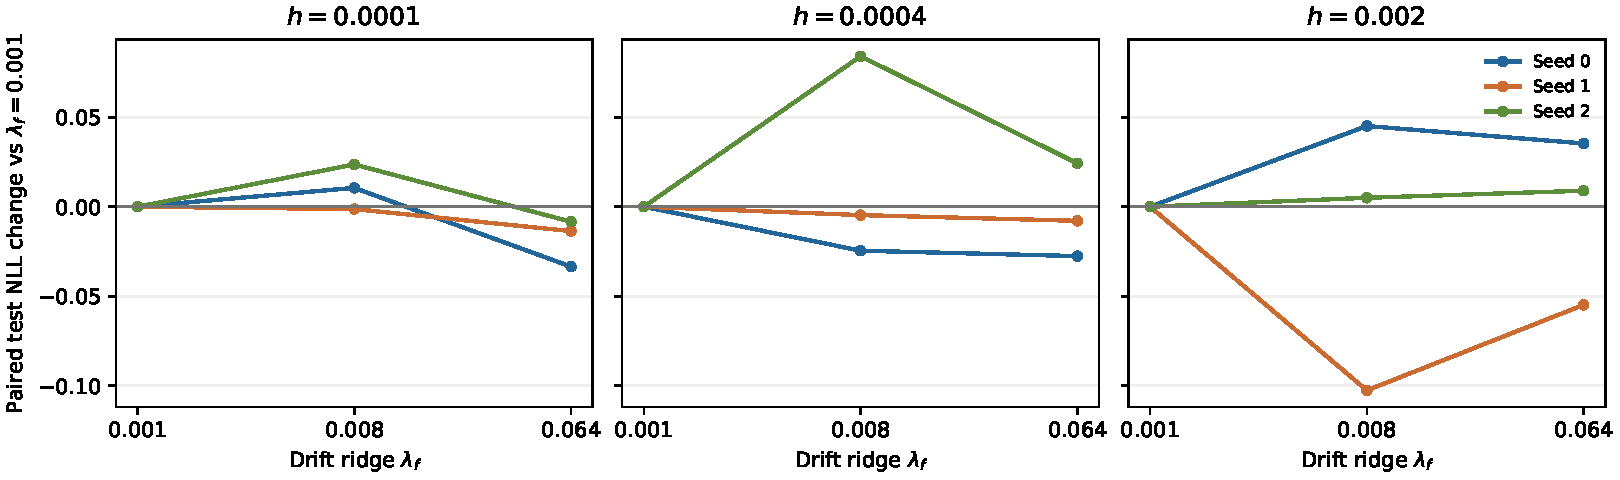
\includegraphics[width=\linewidth]{../figures/lag_ridge_paired_nll.pdf}
\caption{Within-lag paired test NLL changes from $\lambda_f=.001$, with one connected line per fitting seed. The zero at .001 is the same-seed reference, so the lag-dependent density offset does not obscure the intervention. This figure does not select a penalty.}
\label{fig:lag_ridge_nll}\end{figure}

At $h=.002$, $.008$ lowers drift RMSE in all three paired seeds; other drift comparisons are mixed. The larger $.064$ penalty lowers mean drift RMSE at the two shorter lags but worsens one seed at each. Raw covariance RMSE stays near .08 across arms, while raw SPD violations remain common. Paired NLL effects change sign across seeds and lags, except that $.064$ at $h=10^{-4}$ lowers NLL in all three. Final drift checkpoints also change with the penalty; the covariance stage is refitted to each arm's targets. The archived \texttt{per\_run.csv} records all fold/final selected iterations, validation errors, raw minimum eigenvalues and execution scopes. These results do not establish an optimal penalty or a universal benefit, and the ridge intervention was not applied to the production comparisons.

% Proposed appendix after reproducibility appendix. Requires amsmath, graphicx, booktabs.
% Cross-reference from discussion: Appendix~\ref{app:drift_diagnostic}.
\section{A bounded diagnostic of drift estimation error}
\label{app:drift_diagnostic}
This diagnostic explains possible sources of poor drift recovery without changing the production estimator. It uses the Gaussian surrogate
\[
Y=-X+100\sigma(X)\varepsilon,\qquad \varepsilon\sim\mathcal N(0, I_2),
\]
with nominal $h=10^{-4}$, not the canonical finite-lag trajectory data.
The interventions use $N=8192$, fitting subset $n=7373$, $K=1024$ and unnormalized real sine--cosine features. Three algorithm/split repeats share one archived noise pool; they are not three independently generated datasets. Drift MSE averages squared errors over test points and coordinates, and RMSE is its square root per repeat. Expected conditional risk and observed test MSE are distinct quantities.

Condition A freezes frequencies selected with noiseless targets before a noisy amplitude refit. Condition C freezes the first target-independent proposal $\omega_k=0.2Z_k$, $Z_k\sim\mathcal N(0, I_2)$, before target-dependent acceptance. Condition B adapts and selects frequencies using noisy responses. For A/C, exact fixed-design conditional risk separates bias and variance because the frequency choice is independent of the amplitude-fitting noise. That independence does not hold for B.

\begin{table}[ht]
\centering\small
\caption{Means over three paired repeats; distinct risk definitions are not interchangeable. A/C compare $\lambda=.001$ to $.064$. B compares baseline to post-hoc / throughout-path ridge. M/MR both use $\lambda=.064$. Values are rounded only for display.}
\label{tab:drift_diagnostic}
\begin{tabular}{lrrl}\toprule
Comparison & Reference & Intervention & Paired outcome\\\midrule
A: expected conditional MSE & 45.755 & 31.169 & All three improve \\
C: expected conditional MSE & 6.874 & 4.146 & All three improve \\
B: observed test MSE & 16.215 & 9.545 / 10.914 & Post / path ridge \\
M / MR: selected MSE & 10.914 & 6.869 & Two improve, one worsens \\
M / MR: iteration 300 MSE & 124.595 & 616.539 & All three worsen \\
\bottomrule\end{tabular}
\end{table}

For A/C, variance dominates squared bias. Stronger ridge reduces expected and realized error in all six pairs, although the scaled $K=1024$ expected risks remain above their respective $K16$ means (14.607 and 4.017). This is evidence about these bases, not an optimal-ridge rule or a general capacity rate. The normal-equation diagonal shift is $n\lambda$, not $\lambda$.

For B, post-hoc shrinkage on the already selected frequencies reduces observed MSE in all three repeats. Using $.064$ throughout adaptation and checkpoint selection also improves all three relative to baseline, but gives no additional observed benefit over post-hoc shrinkage; repeat 1 is effectively tied (MSE difference $0.000466$). This comparison combines changes to the adaptive path and selection. A noise-independent fixed-basis risk identity cannot be applied to B.

In a separate paired comparison, both arms retain Metropolis updates, $\delta=.2$, $\gamma=1$ and 300 iterations. MR additionally resamples every iteration. The modern update order is proposal, amplitude fit, acceptance, mixed-population refit, optional resampling, and final refit. The earliest strict minimum of noisy internal-validation MSE selects the returned checkpoint; there is no full-data refit. Adding resampling improves two selected models and worsens one. At iteration 300 it worsens all three. The fresh M trajectory is distinct from the archived Bpath trajectory; their close values are not substituted.

\begin{figure}[ht]
\centering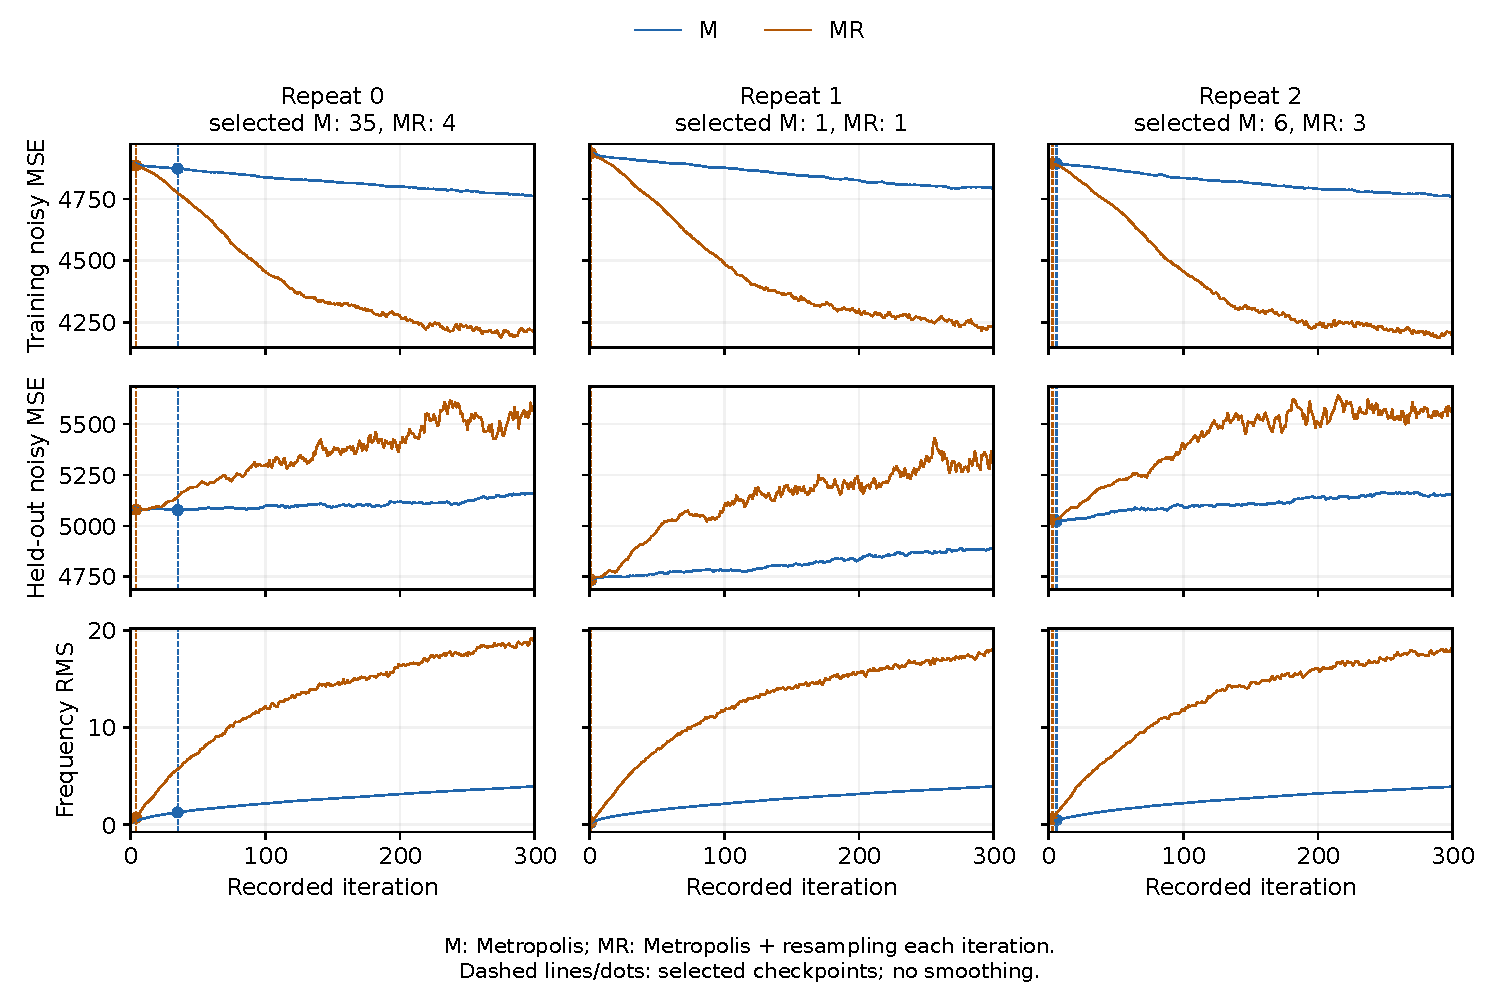
\includegraphics[width=\linewidth]{../figures/mechanism.pdf}
\caption{All recorded training/held-out losses and frequency RMS for all three repeats. Dashed lines and dots mark selected checkpoints. Curves are unsmoothed; frequency RMS includes location as well as spread. Archived centered RMS also grows. No intermediate true-drift errors are inferred.}
\label{fig:drift_diagnostic}
\end{figure}

Training loss decreases overall while held-out noisy loss and frequency spread increase overall; each trajectory has reversals. Selected models have much lower true-drift error than iteration 300. These observations support an overfitting interpretation, but do not prove frequency growth causes it. Noisy checkpoint selection and duplication-induced changes in effective functional regularization remain possible contributors, not isolated causes.

Distinct parent slots are not distinct physical frequencies. Uniform multinomial resampling of 1024 slots already retains only about 647.48 distinct parent slots on average, so observed means near 613 do not establish population collapse. MR's full pre-resampling weights were not archived; ESS alone cannot recover its conditional parent expectation. Higher ESS does not guarantee better recovery.

These results do not establish failure of ESS-triggered resampling, a universal SDE ranking, or an optimal value $.064$. They neither retune the production method nor change production results. The three repeats support these bounded comparisons but do not identify a unique causal mechanism.

\section{Component composition and likelihood calibration}
Post-hoc Joint-MLP-drift/ARFF-covariance composition inherits the component coefficient errors but improves ARFF NLL only modestly. At fixed projected covariance only the quadratic residual term changes. CPU component-swap evaluations are distinct from stored GPU production metrics; float32 and float64 reductions are separate scopes. Their closely rounded values do not denote independent trained models. The instantaneous-coefficient oracle need not optimize finite-lag Gaussian NLL. Fixed-floor sensitivity does not select a replacement production floor.
\begin{table}[ht]\centering\scriptsize\caption{Component-swap CPU evaluations: mean $\pm$ sample SD over 30 seeds. $Q$ is the quadratic term, $D$ the half log-determinant; Gaussian constant $\log(2\pi)=1.837877$. Table~\ref{tab:ex8} instead contains stored production-GPU scores. The float32/float64 blocks agree at four significant digits; paired differences below show their distinct reductions. Identical-oracle roundoff SDs are displayed as zero.}\label{tab:swaps}\begin{tabular}{lrrr}\toprule Combination & $Q$ & $D$ & NLL\\\midrule
\multicolumn{4}{l}{\emph{CPU predictions; float32 projection/likelihood, floor $10^{-3}$}}\\
MLP drift + ARFF cov. & $0.8886\pm 0.0722$ & $-11.64\pm 0.02354$ & $-8.916\pm 0.07438$\\
ARFF drift + ARFF cov. & $0.9074\pm 0.07024$ & $-11.64\pm 0.02354$ & $-8.897\pm 0.07317$\\
True drift + ARFF cov. & $0.8884\pm 0.07218$ & $-11.64\pm 0.02354$ & $-8.916\pm 0.07434$\\
\multicolumn{4}{l}{\emph{CPU predictions; float64 spectral likelihood, floor $10^{-3}$}}\\
MLP drift + ARFF cov. & $0.8886\pm 0.0722$ & $-11.64\pm 0.02354$ & $-8.916\pm 0.07438$\\
ARFF drift + ARFF cov. & $0.9074\pm 0.07024$ & $-11.64\pm 0.02354$ & $-8.897\pm 0.07317$\\
True drift + ARFF cov. & $0.8884\pm 0.07218$ & $-11.64\pm 0.02354$ & $-8.916\pm 0.07434$\\
\multicolumn{4}{l}{\emph{CPU diagnostic; float64, unprojected instantaneous true covariance}}\\
True instantaneous pair & $1.603\times10^{4}\pm 0$ & $-18.42\pm 0$ & $1.602\times10^{4}\pm 0$\\
ARFF drift + true cov. & $1.98\times10^{4}\pm 1947$ & $-18.42\pm 0$ & $1.978\times10^{4}\pm 1947$\\
MLP drift + true cov. & $1.609\times10^{4}\pm 32.45$ & $-18.42\pm 0$ & $1.608\times10^{4}\pm 32.45$\\
\midrule\multicolumn{4}{l}{\emph{Paired CPU float32 minus float64 differences (not new evaluations)}}\\
ARFF drift + ARFF cov. & $-1.609\times10^{-8}\pm 2.323\times10^{-7}$ & $3.116\times10^{-7}\pm 4.146\times10^{-7}$ & $4.112\times10^{-7}\pm 4.87\times10^{-7}$\\
MLP drift + ARFF cov. & $-2.246\times10^{-8}\pm 2.17\times10^{-7}$ & $3.116\times10^{-7}\pm 4.146\times10^{-7}$ & $5.281\times10^{-7}\pm 3.902\times10^{-7}$\\
True drift + ARFF cov. & $-2.537\times10^{-8}\pm 2.306\times10^{-7}$ & $3.116\times10^{-7}\pm 4.146\times10^{-7}$ & $4.795\times10^{-7}\pm 4.794\times10^{-7}$\\
\bottomrule\end{tabular}\end{table}
\begin{table}[ht]\centering\small\caption{Post-hoc float64 floor sensitivity; no floor is selected. All 30 seeds and all prescribed floors retained. Raw covariance RMSE is unchanged. Projected RMSE is shared by the three drift choices.}\begin{tabular}{rrlll}\toprule Floor & Projected cov. RMSE & True drift NLL & MLP drift NLL & ARFF drift NLL\\\midrule
$1\times10^{-8}$ & $0.1129\pm 0.002269$ & $3.327\times10^{4}\pm 6672$ & $3.329\times10^{4}\pm 6673$ & $3.502\times10^{4}\pm 6476$\\
$1\times10^{-6}$ & $0.1129\pm 0.002269$ & $322\pm 66.72$ & $322.2\pm 66.74$ & $339.6\pm 64.77$\\
0.0001 & $0.1129\pm 0.002269$ & $-6.436\pm 0.6757$ & $-6.434\pm 0.6759$ & $-6.258\pm 0.6572$\\
0.001 & $0.1129\pm 0.002269$ & $-8.916\pm 0.07434$ & $-8.916\pm 0.07438$ & $-8.897\pm 0.07317$\\
\bottomrule\end{tabular}\end{table}

